%!TEX program = xelatex
%Template created by: Maciej Byczko
\documentclass[a4paper,12pt]{extarticle}  %typ dokumentu

\usepackage{geometry} %poprawienie marginesów
\usepackage{polski} %polskie znaki
\usepackage{graphicx} %grafiki
\usepackage{multirow} % tabele
\usepackage{bigstrut} % tabele
\usepackage{float} %poprawienie pozycji
\usepackage{fancyhdr} % header i footer
\usepackage{hyperref} %tworzenie odnośników, \url{<url>}, \href{<file path, link>}{<text with link>} \pageref{}
\usepackage{slashbox}
% \usepackage{multirow}
% \usepackage{tocbibind}
\graphicspath{{pictures/}}
\geometry{margin=0.7in}
\pagestyle{fancy}
\cfoot{Strona \thepage}
\rhead{Strona \thepage}
\lhead{\typdoc}
\setlength{\headheight}{15pt}

%Ustawienie paczki hyperref
\hypersetup{
     colorlinks,
     citecolor=black,
     filecolor=black,
     linkcolor=black,
     urlcolor=black
}


\title{\tytul \\ \small{\opis}}
\author{\tworcy}
\date{\data}

%-----------------------SEKCJA DANYCH----------------------------------
\def\tytul{Technologie Sieciowe - Projekt} %<<< tytuł ćwiczenia
\def\nrcw{} %<<< numer ćwiczenia
\def\data{\today \\ \small{\zajinfo}} %<< data wykonania
\def\prowadzacy{Prowadzący: dr. inż Arkadiusz Grzybowski} %<<<prowadzący
\def\nrgrupy{} %<<<numer grupy
\def\tworcy{Autorzy:\\Karol Baraniecki (252726)\\Maciej Byczko(252747)} %<<< autorzy
\def\zajinfo{PN 14:00 TP\\ Politechnika Wrocławska\\Wydział Informatyki i Telekomunikacji} %<<< informacje dotyczące zajęć
\def\typdoc{} %<<< typ dokumentu tj Sprawozdanie, zadania itp. {Matematyka dyskretna/Sprawozdanie z Miernictwa}
\def\opis{\prowadzacy} %<<< opis który będzie umieszczony pod tytułem w Maketitle
%----------------------------------------------------------------------


\begin{document}
\maketitle
\tableofcontents
\listoftables
\cleardoublepage
\section{Wstęp}
Celem projektu jest zaprojektowanie lokalnej sieci komputerowej dla firmy programistycznej znajdującej się we Wrocławiu.
Sieć musi zostać zaprojektowana zgodnie ze sprecyzowanymi wymaganiami firmy oraz uwzględniać jej przyszły rozwój.
\subsection{Kadra firmy}

W personel firmy składa się z następujących użytkowników:
\begin{itemize}\label{itemize:kadra}
	\item Programiści
	\item Testerzy
	\item Projektanci
	\item Marketing
	\item Księgowość
\end{itemize}
\subsection{Opis siedziby firmy}
Przedsiębiorstwo znajduje się przy ulicy Nowowiejskiej 69\label{address}, składa się z dwóch budynków: dwupiętrowego oraz trzypiętrowego.
W budynkach znajduje się także odpowiednie wyposażenie (serwery,  drukarki,
komputery,  kamery  IP,  itp.).
Firma posiada jeden główny punkt dystrybucyjny (MDF) oraz punkty pośrednie (IDF) w każdym z budynków.
\subsubsection{Lokalizacja firmy na mapie}
\begin{minipage}[c]{0.49\linewidth}
	
	\begin{figure}[H]
		\centering
		\resizebox*{\textwidth}{!}{
			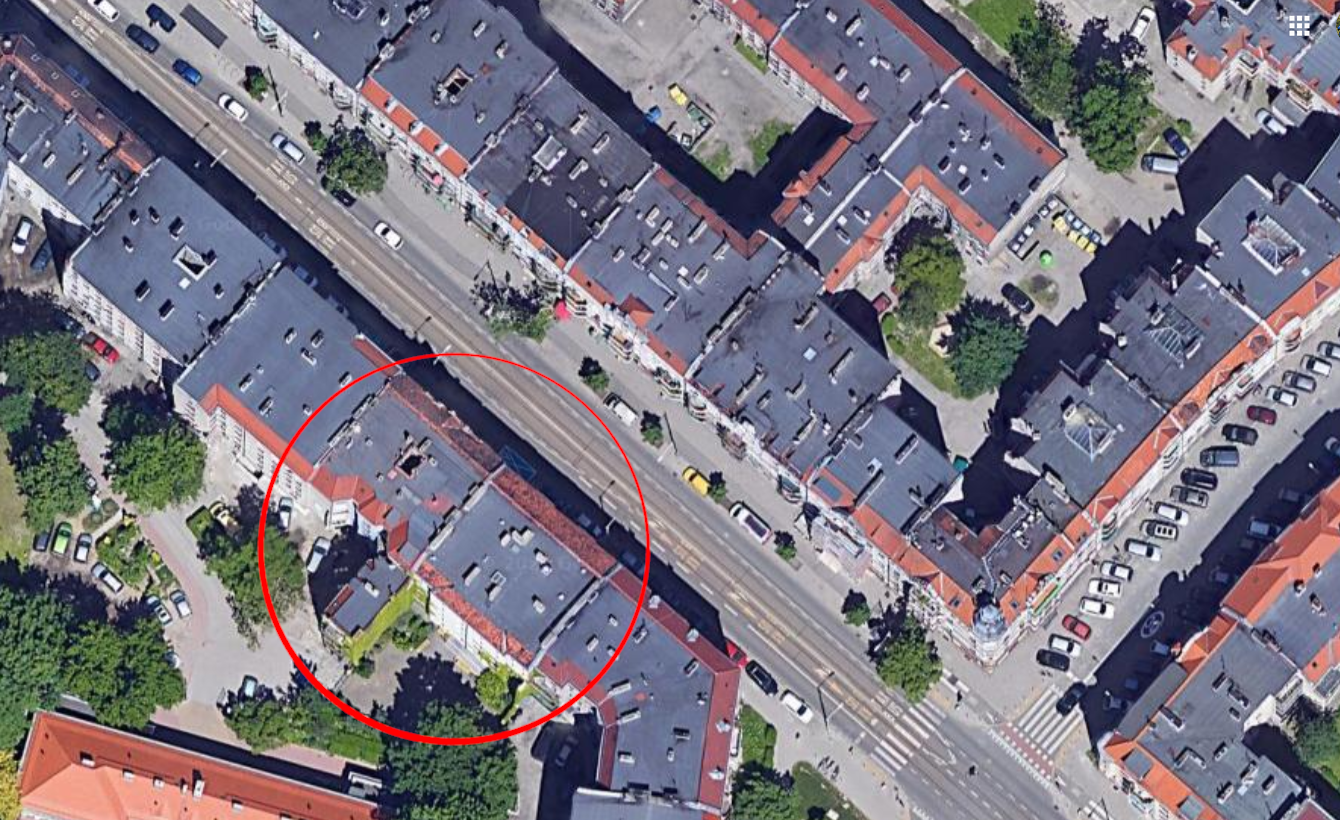
\includegraphics{../pictures/building_close.png}
			}
		\end{figure}
\end{minipage}
\begin{minipage}[c]{0.49\linewidth}
	
	\begin{figure}[H]
		\centering
		\resizebox*{\textwidth}{!}{
			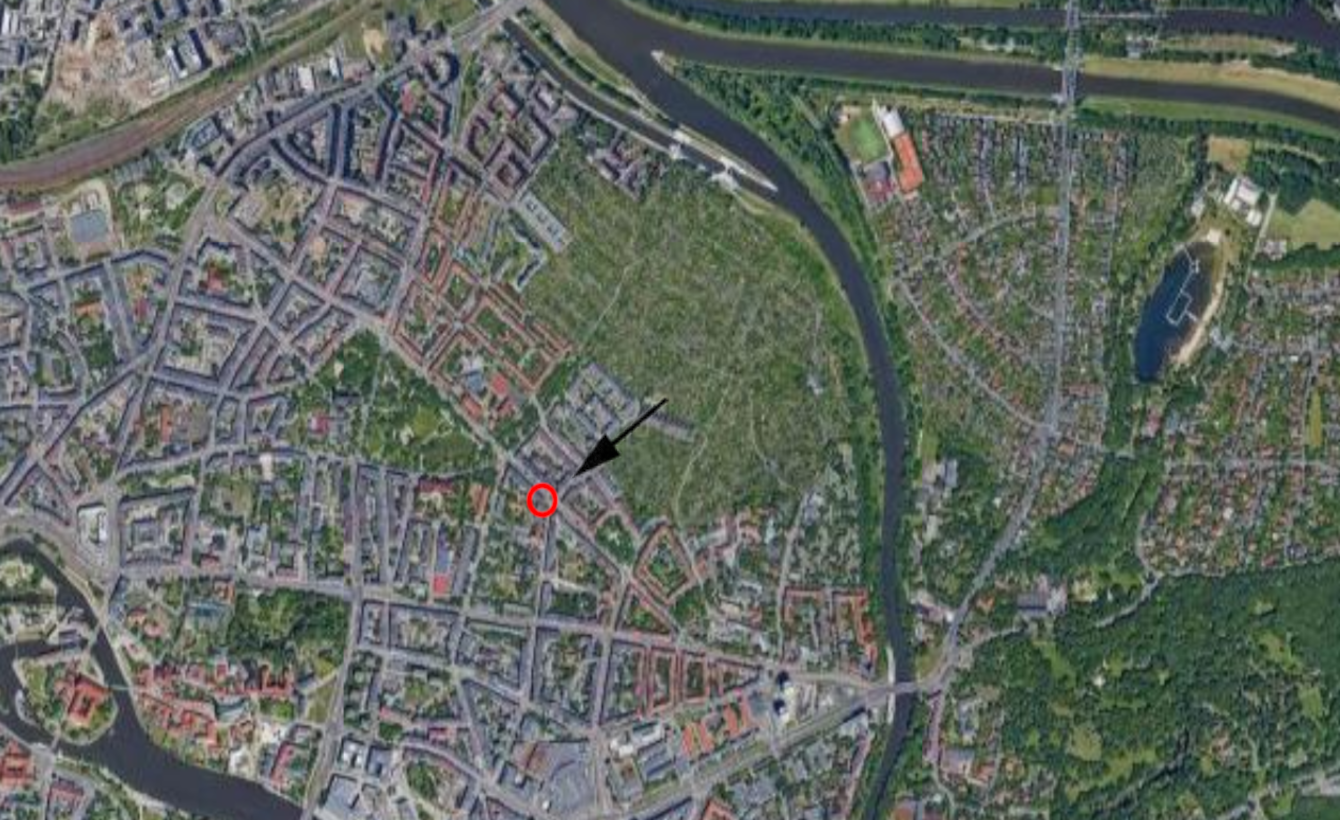
\includegraphics{../pictures/building_not_close.png}
			}
		\end{figure}
\end{minipage}
\subsection{Wymagania}
Firma wymaga od nas aby:
\begin{itemize}
	\item Użyta technologia była z rodziny Ethernet,
	\item na wskazanym piętrze każdego budynku ma być dostępna sieć bezprzewodowa (niezbędna instalacja
	      kablowa jest przygotowana),
	\item należy zapewnić dodatkowe porty na przełącznikach (w liczbie 20\% zajętych portów), w związku z
	      przewidywanym wzrostem liczby pracowników (w pomieszczeniach są już zainstalowane
	      dodatkowe gniazda sieciowe),
	\item ruch w ramach grup roboczych ma być separowany z wykorzystaniem sieci VLAN,
	\item należy  zapewnić  dwa  podłączenia  do  Internetu:  podstawowe  oraz  zapasowe,  o  przepustowości
	      adekwatnej do potrzeb przedsiębiorstwa,
	\item podstawowe  łącze  internetowe  ma  zapewniać  gwarancję  minimalnej  przepustowości  równej  co
	      najmniej 40\% średniego przewidywanego przepływu na tym łączu,
	\item kosztorys ma uwzględniać koszt wszystkich urządzeń, podłączenia do Internetu i koszt korzystania z
	      łączy Internetowych w okresie 2 lat
\end{itemize}


%!=========ETAP 2=============


\section{Inwentaryzacja zasobów}
Ilości posiadanych pracowników, oraz urządzeń.
\subsection{Pracownicy}
Pracowników można podzielić na 5 grup roboczych (Patrz \underline{\nameref{itemize:kadra}}).
Każdy z pracowników posiada dostęp do stanowiska pracy na którym znajduje się urządzenie wymagające podłączenia do sieci (w naszym przypadku każdy użytkownik posiada komputer)

\subsubsection{Tabele podziału pracowników}
\begin{table}[H]
	\centering
	\caption{Podział użytkowników na grupy robocze, budynki oraz piętra}
	\vspace{2mm}
	\resizebox{\textwidth}{!}{
		\begin{tabular}{|c|c|c|c|c|c|}
			\cline{2-6}    \multicolumn{1}{c|}{} & \multicolumn{5}{c|}{\textbf{Liczba użytkowników (komputerów)}} \bigstrut                                                                                                                           \\
			\cline{2-6}    \multicolumn{1}{c|}{} & \multicolumn{2}{c|}{\textbf{Budynek 1}}                                  & \multicolumn{3}{c|}{\textbf{Budynek 2}} \bigstrut                                                                       \\\hline
			\textbf{Grupa robocza}               & \textbf{Piętro 1}                                                        & \textbf{Piętro 2}                                 & \textbf{Piętro 1} & \textbf{Piętro 2} & \textbf{Piętro 3} \bigstrut \\\hline
			\textbf{Programiści}                 & 22                                                                       & 6                                                 & 2                 & 19                & 36 \bigstrut                \\\hline
			\textbf{Testerzy}                    & 21                                                                       & 31                                                & 6                 & 13                & 33 \bigstrut                \\\hline
			\textbf{Projektanci}                 & 6                                                                        & 31                                                & 18                & 1                 & 14 \bigstrut                \\\hline
			\textbf{Marketing}                   & 16                                                                       & 28                                                & 7                 & 3                 & 17 \bigstrut                \\\hline
			\textbf{Księgowość}                  & 32                                                                       & 14                                                & 32                & 21                & 15 \bigstrut                \\\hline
		\end{tabular}%
	}
	\label{tab:groups}%
\end{table}%

\begin{table}[H]
	\centering
	\caption{Suma poszczególnych pracowników w firmie wraz z podziałem na grupy robocze}
	\vspace{2mm}
	\begin{tabular}{|c|r|}\hline
		\textbf{Grupa robocza}               & \multicolumn{1}{l|}{\textbf{Suma}} \bigstrut \\\hline
		\textbf{Programiści}                 & 85 \bigstrut                                 \\\hline
		\textbf{Testerzy}                    & 104 \bigstrut                                \\\hline
		\textbf{Projektanci}                 & 70 \bigstrut                                 \\\hline
		\textbf{Marketing}                   & 71 \bigstrut                                 \\\hline
		\textbf{Księgowość}                  & 114 \bigstrut                                \\\hline
		\textbf{Liczba drukarek}             & 12 \bigstrut                                 \\\hline
		\textbf{Suma wszystkich pracowników} & 444 \bigstrut                                \\\hline
	\end{tabular}%
	\label{tab:groups_sum}%
\end{table}%

\subsection{Sprzęt}
Firma jest wyposażona w trzy rodzaje sprzętu:
\begin{itemize}
	\item drukarki
	\item punkty dostępowe WiFi
	\item urządzenia bezprzewodowe
\end{itemize}
Sprzęty te będą używane w sieci lokalnej firmy.
\subsubsection{Tabele podziału urządzeń wspólnych}
\begin{table}[H]
	\centering
	\caption{Podział urządzeń na budynki oraz piętra}
	\vspace{2mm}
	\resizebox{\textwidth}{!}{
		\begin{tabular}{|c|c|c|c|c|c|}
			\cline{2-6}    \multicolumn{1}{c|}{}     & \multicolumn{5}{c|}{\textbf{Liczba urządzeń}} \bigstrut                                                                                                                           \\
			\cline{2-6}    \multicolumn{1}{c|}{}     & \multicolumn{2}{c|}{\textbf{Budynek 1}}                 & \multicolumn{3}{c|}{\textbf{Budynek 2}} \bigstrut                                                                       \\\hline
			\textbf{Urządzenia}                      & \textbf{Piętro 1}                                       & \textbf{Piętro 2}                                 & \textbf{Piętro 1} & \textbf{Piętro 2} & \textbf{Piętro 3} \bigstrut \\\hline
			\textbf{Liczba drukarek}                 & 1                                                       & 2                                                 & 3                 & 3                 & 3 \bigstrut                 \\\hline
			\textbf{Liczba punktów dostępowych WiFi} & 0                                                       & 0                                                 & 1                 & 0                 & 3 \bigstrut                 \\\hline
			\textbf{Liczba urządzeń bezprzewodowych} & 0                                                       & 0                                                 & 6                 & 0                 & 17 \bigstrut                \\\hline
		\end{tabular}%
	}
	\label{tab:devices}%
\end{table}%

\begin{table}[H]
	\centering
	\caption{Suma poszczególnych urządzeń w firmie}
	\vspace{2mm}
	\begin{tabular}{|c|r|}\hline
		\textbf{Urządzenia}                      & \multicolumn{1}{l|}{\textbf{Suma}} \bigstrut \\\hline
		\textbf{Liczba drukarek}                 & 12 \bigstrut                                 \\\hline
		\textbf{Liczba punktów dostępowych WiFi} & 4 \bigstrut                                  \\\hline
		\textbf{Liczba urządzeń bezprzewodowych} & 23 \bigstrut                                 \\\hline
		\textbf{Suma wszystkich urządzeń}        & 39 \bigstrut                                 \\\hline
	\end{tabular}%
	\label{tab:devices_sum}%
\end{table}%

\subsubsection{Wymagania przepływowe pomiędzy pracownikami a serwerami lokalnymi}


\subsubsection{Serwery}
Firma posiada dwa serwery lokalne. Serwer lokalny 1 jest używany przez:
\begin{itemize}
	\item Testerów,
	\item Marketing,
	\item WiFi
\end{itemize}
Serwer lokalny 2 jest używany przez każdą grupę roboczą z wyłączeniem zespołu Marketingu.
\begin{table}[H]
	\centering
	\caption{Prognozowany ruch do internetu}
	\vspace{2mm}
	\resizebox{\textwidth}{!}{
		\begin{tabular}{|c|c|c|c|}
			\cline{2-4}    \multicolumn{1}{c|}{} & \multicolumn{3}{c|}{\textbf{Transfer do\textbackslash{}z Internetu na jedną sesję (internautę) [kb/s] }} \bigstrut                                                                        \\\hline
			\textbf{Serwery internetowe}         & \textbf{Do Internetu}                                                                                              & \textbf{Z Internetu} & \textbf{Liczba jednoczesnych sesji} \bigstrut \\\hline
			\textbf{Serwer WWW}                  & 50                                                                                                                 & 15                   & 49 \bigstrut                                  \\\hline
			\textbf{Serwer FTP}                  & 210                                                                                                                & 90                   & 4 \bigstrut                                   \\\hline
		\end{tabular}%
	}
	\label{tab:www_traffic}%
\end{table}%
\subsection{Aplikacje}
Dla każdej grupy użytkowników został zdefiniowany również przepływ do i z internetu z podziałem na poszczególne typy aplikacji, firma zapewnia również dostęp do sieci WiFi.
\begin{table}[H]
	\centering
	\caption{Wymagania dotyczące przepływu przez aplikacje}
	\vspace{2mm}
	\resizebox{\textwidth}{!}{
		\begin{tabular}{|c|c|c|c|c|c|}\hline
			\multicolumn{6}{|c|}{\textbf{Transfer z/do Internetu (down \textbackslash{} up) [kb/s]}} \bigstrut                                                                               \\\hline
			\textbf{\backslashbox{Grupa rob.}{Aplikacja}} & \textbf{Przeglądarka} & \textbf{Wideokonferencja} & \textbf{VoIP}        & \textbf{Klient\_FTP} & \textbf{Komunikator} \bigstrut \\\hline
			\textbf{Programiści}                          & 0\textbackslash{}0    & 0\textbackslash{}0        & 20\textbackslash{}20 & 77\textbackslash{}18 & 15\textbackslash{}15 \bigstrut \\\hline
			\textbf{Testerzy}                             & 0\textbackslash{}0    & 40\textbackslash{}40      & 0\textbackslash{}0   & 0\textbackslash{}0   & 15\textbackslash{}15 \bigstrut \\\hline
			\textbf{Projektanci}                          & 65\textbackslash{}10  & 0\textbackslash{}0        & 20\textbackslash{}20 & 45\textbackslash{}11 & 15\textbackslash{}15 \bigstrut \\\hline
			\textbf{Marketing}                            & 60\textbackslash{}10  & 40\textbackslash{}40      & 20\textbackslash{}20 & 0\textbackslash{}0   & 15\textbackslash{}15 \bigstrut \\\hline
			\textbf{Księgowość}                           & 35\textbackslash{}10  & 40\textbackslash{}40      & 20\textbackslash{}20 & 0\textbackslash{}0   & 0\textbackslash{}0 \bigstrut   \\\hline
			\textbf{WiFi}                                 & 78\textbackslash{}10  & 40\textbackslash{}40      & 20\textbackslash{}20 & 49\textbackslash{}14 & 15\textbackslash{}15 \bigstrut \\\hline
		\end{tabular}%
	}
	\label{tab:apps}%
\end{table}%

\section{Analiza potrzeb użytkowników}
Wymagania potrzebne dla pracowników w celu sprawnej pracy w firmie.
\subsection{Pracownicy oraz wykorzystywane oprogramowanie}
W zależności od typu stanowiska wymagana jest różna jakość usług sieciowych. Jest to związane z tym że wykorzystywane jest różne oprogramowanie. Każda aplikacja działa w sposób indywidualny, niektóre wymagają bardzo stabilnego łącza, bądź bezpieczeństwa połączenia.
Na podstawie \underline{\hyperref[tab:usage]{tabeli 7}} można wywnioskować wymagania oraz zużycie każdej grupy roboczej, rozpatrzymy każde stanowisko z osobna:
\begin{itemize}
	\item Programiści - wymagają przede wszystkim szybkiego połączenia ze względu na znaczne użycie usługi FTP.
	\item Testerzy - wymagają szybkiego i niezawodnego łącza ze względu na wideokonferencje.
	\item Projektanci - wymagają bezpiecznego oraz szybkiego połączenia ze względu na usługę FTP oraz używanie przeglądarki.
	\item Marketing - wymagają stabilnego łącza ze względu na wideokonferencję, bezpieczeństwo także się przyda ze względu na użycie przeglądarki.
	\item Księgowość - głównie wymagają stabilnego łącza ze względu na wideokonferencje, używają także przeglądarki więc łącze musi być bezpieczne.
	      % \item WiFi - oferuje multum usług więc powinno mieć głównie bezpieczeństwo połączenia,  
\end{itemize}

\subsection{Łącza szkieletowe}
% \subsection{Łącza do serwerów i drukarek}
\begin{table}[H]
	\centering
	\caption{Wymagania dotyczące przepływów lokalnych (na jednego użytkownika)}
	\vspace{2mm}
	\resizebox{\textwidth}{!}{
		\begin{tabular}{|c|c|c|c|}
			\cline{2-4}    \multicolumn{1}{c|}{}       & \multicolumn{3}{c|}{\textbf{Transfer do serwerów lokalnych i drukarek (down \textbackslash{} up) [kb/s]}} \bigstrut                                                            \\\hline
			\textbf{\backslashbox{Grupa rob.}{Serwer}} & \textbf{Serwer1}                                                                                                    & \textbf{Serwer2}       & \textbf{Drukarka} \bigstrut     \\\hline
			\textbf{Programiści}                       & 0\textbackslash{}0                                                                                                  & 750\textbackslash{}700 & 10\textbackslash{}120 \bigstrut \\\hline
			\textbf{Testerzy}                          & 700\textbackslash{}350                                                                                              & 450\textbackslash{}100 & 10\textbackslash{}130 \bigstrut \\\hline
			\textbf{Projektanci}                       & 0\textbackslash{}0                                                                                                  & 350\textbackslash{}200 & 10\textbackslash{}190 \bigstrut \\\hline
			\textbf{Marketing}                         & 150\textbackslash{}200                                                                                              & 0\textbackslash{}0     & 10\textbackslash{}140 \bigstrut \\\hline
			\textbf{Księgowość}                        & 0\textbackslash{}0                                                                                                  & 450\textbackslash{}250 & 10\textbackslash{}130 \bigstrut \\\hline
			\textbf{WiFi}                              & 50\textbackslash{}250                                                                                               & 100\textbackslash{}250 & 10\textbackslash{}120 \bigstrut \\\hline
		\end{tabular}%
	}
	\label{tab:usage}%
\end{table}%
Aby uzyskać szacowane łącza według grup roboczych na jednego użytkownika należy zsumować cały ruch generowany przez jednego użytkownika danej grupy.
Wyliczenia zostały wykonane na podstawie poprzednich tabel.

\begin{table}[H]
	\centering
	\caption{Szacowane wykorzystywanie łącza przez pojedynczego użytkownika z danych grup roboczych}
	\vspace{2mm}
	\resizebox{\textwidth}{!}{
		\begin{tabular}{|c|c|c|c|c|c|c|}
			\hline
			\multirow{3}[4]{*}{\textbf{Użytkownik}} & \multicolumn{2}{c|}{\textbf{Lokalnie}} & \multicolumn{2}{c|}{\textbf{Internet}} & \multicolumn{2}{c|}{\textbf{Suma}} \bigstrut                                                                    \\
			\cline{2-7}                             & \textbf{down}                          & \textbf{up}                            & \textbf{down}                                & \textbf{up}     & \textbf{down}   & \textbf{up} \bigstrut[t]     \\
			                                        & \textbf{[kb/s]}                        & \textbf{[kb/s]}                        & \textbf{[kb/s]}                              & \textbf{[kb/s]} & \textbf{[kb/s]} & \textbf{[kb/s]} \bigstrut[b] \\\hline
			\textbf{Programiści}                    & 760                                    & 820                                    & 112                                          & 53              & 872             & 873 \bigstrut                \\\hline
			\textbf{Testerzy}                       & 1160                                   & 580                                    & 55                                           & 55              & 1215            & 635 \bigstrut                \\\hline
			\textbf{Projektanci}                    & 360                                    & 390                                    & 145                                          & 56              & 505             & 446 \bigstrut                \\\hline
			\textbf{Marketing}                      & 160                                    & 340                                    & 135                                          & 85              & 295             & 425 \bigstrut                \\\hline
			\textbf{Księgowość}                     & 460                                    & 380                                    & 95                                           & 70              & 555             & 450 \bigstrut                \\\hline
			\textbf{WiFi}                           & 160                                    & 620                                    & 202                                          & 99              & 362             & 719 \bigstrut                \\\hline
		\end{tabular}%
	}
	\label{tab:user_usage}%
\end{table}%
\textbf{Przykład obliczeń:}\\
Wyliczenia na podstawie grupy roboczej \emph{Programiści} z \underline{\hyperref[tab:apps]{tabeli 7}}:
\begin{itemize}
	\item Pobieranie z Internetu: $0+0+20+77+15=112[kb/s]$
	\item Wysyłanie do Internetu: $0+0+20+18+15=53[kb/s]$
	\item Pobieranie lokalne: $0+750+10=760[kb/s]$
	\item Wysyłanie lokalne:$0+700+120=820[kb/s]$
	\item Suma pobierania: $112+760=872[kb/s]$
	\item Suma wysyłania: $53+820=873[kb/s]$
\end{itemize}
Grupy o największym korzystaniu z sieci to:
\begin{itemize}
	\item Testerzy (Pobieranie) - $1215[kb/s] \approx 1.19[Mb/s]$
	\item Programiści (Wysyłanie) - $873[kb/s] \approx 0.85[Mb/s]$ %(po zaokrągleniu w górę $0.86[Mb/s]$ aby nie było straty na łączu)
\end{itemize}
Aby uzyskać szacowany ruch generowany przez pracowników danego piętra,
należy pomnożyć ruch przypadający na jednego pracownika z
\underline{\hyperref[tab:user_usage]{tabeli 8}} przez liczbę pracowników danej grupy roboczej na określonym piętrze (\underline{\hyperref[tab:groups]{tabela 1}})
% \subsubsection{Szacowany pobór danych}
% Table generated by Excel2LaTeX from sheet 'Sheet1'
% Table generated by Excel2LaTeX from sheet 'Sheet1'
\begin{table}[H]
	\centering
	\caption{Szacowany pobór danych}
	\vspace{2mm}
	\resizebox{\textwidth}{!}{
		\begin{tabular}{|c|c|c|c|c|c|}
			\hline
			\multirow{2}[4]{*}{\textbf{Użytkownik}} & \multicolumn{2}{c|}{\textbf{Budynek 1}} & \multicolumn{3}{c|}{\textbf{Budynek 2}} \bigstrut                                                                       \\
			\cline{2-6}                             & \textbf{Piętro 1}                       & \textbf{Piętro 2}                                 & \textbf{Piętro 1} & \textbf{Piętro 2} & \textbf{Piętro 3} \bigstrut \\
			\hline
			\textbf{Programiści}                    & 19184                                   & 5232                                              & 1744              & 16568             & 31392 \bigstrut             \\
			\hline
			\textbf{Testerzy}                       & 25515                                   & 37665                                             & 7290              & 15795             & 40095 \bigstrut             \\
			\hline
			\textbf{Projektanci}                    & 3030                                    & 15655                                             & 9090              & 505               & 7070 \bigstrut              \\
			\hline
			\textbf{Marketing}                      & 4720                                    & 8260                                              & 2065              & 885               & 5015 \bigstrut              \\
			\hline
			\textbf{Księgowość}                     & 17760                                   & 7770                                              & 17760             & 11655             & 8325 \bigstrut              \\
			\hline
			\textbf{Suma}                           & 70209                                   & 74582                                             & 37949             & 45408             & 91897 \bigstrut             \\
			\hline
		\end{tabular}%
	}
	\label{tab:user_download}%
\end{table}%

% Table generated by Excel2LaTeX from sheet 'Sheet1'
\begin{table}[H]
	\centering
	\caption{Szacowany przesył danych
		\vspace{2mm}}
	\resizebox{\textwidth}{!}{
		\begin{tabular}{|c|c|c|c|c|c|}
			\hline
			\multirow{2}[4]{*}{\textbf{Użytkownik}} & \multicolumn{2}{c|}{\textbf{Budynek 1}} & \multicolumn{3}{c|}{\textbf{Budynek 2}} \bigstrut                                                                       \\
			\cline{2-6}                             & \textbf{Piętro 1}                       & \textbf{Piętro 2}                                 & \textbf{Piętro 1} & \textbf{Piętro 2} & \textbf{Piętro 3} \bigstrut \\
			\hline
			\textbf{Programiści}                    & 19206                                   & 5238                                              & 1746              & 16587             & 31428 \bigstrut             \\
			\hline
			\textbf{Testerzy}                       & 13335                                   & 19685                                             & 3810              & 8255              & 20955 \bigstrut             \\
			\hline
			\textbf{Projektanci}                    & 2676                                    & 13826                                             & 8028              & 446               & 6244 \bigstrut              \\
			\hline
			\textbf{Marketing}                      & 6800                                    & 11900                                             & 2975              & 1275              & 7225 \bigstrut              \\
			\hline
			\textbf{Księgowość}                     & 14400                                   & 6300                                              & 14400             & 9450              & 6750 \bigstrut              \\
			\hline
			\textbf{Suma}                           & 56417                                   & 56949                                             & 30959             & 36013             & 72602 \bigstrut             \\
			\hline
		\end{tabular}%
	}
	\label{tab:user_upload}%
\end{table}%
\textbf{Przykład obliczeń:}\\
Wyliczenia na podstawie grupy roboczej \emph{Programiści} z \underline{\hyperref[tab:user_usage]{tabeli 8}} oraz \underline{\hyperref[tab:groups]{tabeli 1}}:\\
Dla piętra 1:
\begin{itemize}
	\item Pobieranie: $872*22=19184[kb/s]\approx 18.74[Mb/s]$
	\item Wysyłanie: $873*22=19206[kb/s]\approx 18.76[Mb/s]$
\end{itemize}
Według przeprowadzonych obliczeń najbardziej wymagające jest \textbf{Piętro 3 w budynku 2}.
\begin{itemize}
	\item Pobieranie: $91897[kb/s]\approx89.75[Mb/s]$
	\item Wysyłanie: $72602[kb/s]\approx70.90[Mb/s]$
\end{itemize}
\subsection{Obciążenie poszczególnych punktów dystrybucyjnych}
% Table generated by Excel2LaTeX from sheet 'Sheet1'
\begin{table}[H]
	\centering
	\caption{Punkty dystrybucyjne i ich obciążenie}
	\resizebox{\textwidth}{!}{
		\begin{tabular}{|c|c|c|c|c|}
			\hline
			\multicolumn{3}{|c|}{\textbf{Punkty dystrybucyjne}} & \multicolumn{2}{c|}{\textbf{Transmisja}} \bigstrut                                                                                                                   \\
			\hline
			\textbf{Oznaczenie}                                 & \textbf{Lokalizacja}                               & \textbf{Podłączone punkty abonenckie} & \textbf{Pobór danych [Mb/s]} & \textbf{Przesył danych [Mb/s]} \bigstrut \\
			\hline
			\textbf{MDF}                                        & Bud. 2, Piętro 2                                   & Bud. 2, Piętro 2,1,                   & 312.54                       & 247.01 \bigstrut                         \\
			\hline
			\textbf{IDF1}                                       & Bud. 2, Piętro 3                                   & Bud. 2, Piętro 3,                     & 89.74                        & 70.90 \bigstrut                          \\
			\hline
			\textbf{IDF2}                                       & Bud. 1, Piętro 1                                   & Bud. 1                                & 141.40                       & 110.71 \bigstrut                         \\
			\hline
		\end{tabular}%
	}
	\label{tab:distribution}%
\end{table}%
Na podstawie powyższej tabeli możemy określić że największe obciążenie sieci będzie wynosić kolejno:
Pobór w wysokości 312.54[Mb/s] oraz Przesył w wysokości 247.01[Mb/s],
zatem te wartości uznajemy za wymagania naszej sieci.
\subsection{Łącza do serwerów i drukarek}
Aby uzyskać przepustowości połączeń do serwerów lokalnych oraz drukarek
(zakładając, że są dostępne dla dużej ilości użytkowników jednocześnie)
należy pomnożyć ilość pracowników każdej z grup roboczych (\href{tab:groups_sum}{Tabela 2})
przez wymaganą szybkość połączenia z danym serwerem (\underline{\href{tab:usage}{Tabela 7}}).
Tak uzyskane wyniki przedstawiamy w tabeli reprezentującej przepustowości dla każdej z grup
roboczych oraz ich łączną sumę:
% Table generated by Excel2LaTeX from sheet 'Sheet1'
\begin{table}[H]
	\centering
	\caption{Szacowane przepustowości połączeń poboru danych z serwerów i drukarek}
	\resizebox{\textwidth}{!}{
		\begin{tabular}{|c|c|c|c|c|}
			\hline
			\textbf{\backslashbox{Grupa rob.}{Serwer}} & \textbf{Serwer} 1 & \textbf{Serwer} 2 & \textbf{Drukarka} & \textbf{suma} \bigstrut \\
			\hline
			\textbf{Programiści}                       & 0                 & 63750             & 850               & 64600 \bigstrut         \\
			\hline
			\textbf{Testerzy}                          & 72800             & 46800             & 1040              & 120640 \bigstrut        \\
			\hline
			\textbf{Projektanci}                       & 0                 & 24500             & 700               & 25200 \bigstrut         \\
			\hline
			\textbf{Marketing}                         & 10650             & 0                 & 710               & 11360 \bigstrut         \\
			\hline
			\textbf{Księgowość}                        & 0                 & 51300             & 1140              & 52440 \bigstrut         \\
			\hline
			\textbf{WiFi}                              & 200               & 400               & 40                & 640 \bigstrut           \\
			\hline
		\end{tabular}%
	}
	\label{tab:server_download}%
\end{table}%
\begin{table}[H]
	\centering
	\caption{Szacowane przepustowości przesyłu danych do serwerów i drukarek}
	\resizebox{\textwidth}{!}{
		\begin{tabular}{|c|c|c|c|c|}
			\hline
			\textbf{\backslashbox{Grupa rob.}{Serwer}} & \textbf{Serwer} 1 & \textbf{Serwer} 2 & \textbf{Drukarka} & \textbf{suma} \bigstrut \\
			\hline
			\textbf{Programiści}                       & 0                 & 59500             & 10200             & 69700 \bigstrut         \\
			\hline
			\textbf{Testerzy}                          & 36400             & 10400             & 13520             & 60320 \bigstrut         \\
			\hline
			\textbf{Projektanci}                       & 0                 & 14000             & 13300             & 27300 \bigstrut         \\
			\hline
			\textbf{Marketing}                         & 14200             & 0                 & 9940              & 24140 \bigstrut         \\
			\hline
			\textbf{Księgowość}                        & 0                 & 28500             & 14820             & 43320 \bigstrut         \\
			\hline
			\textbf{WiFi}                              & 1000              & 1000              & 480               & 2480 \bigstrut          \\
			\hline
		\end{tabular}%
	}
	\label{tab:server_upload}%
\end{table}%

\subsection{Łącza do internetu}
Łącze internetowe w firmie będzie wykorzystywane przez aplikacje pracowników oraz z
zewnątrz do dostępu do Serwera WWW oraz Serwera Pocztowego.
Aby obliczyć wykorzystanie łącza internetowego należy pomnożyć przepustowości
wymagane dla danych aplikacji (Tabela \underline{\href{tab:apps}{Tabela 6}}) przez ilość pracowników w każdej
z grup roboczych (\underline{\href{tab:groups_sum}{Tabela 2}} i \underline{\href{tab:devices_sum}{Tabela 4}}):
% Table generated by Excel2LaTeX from sheet 'Sheet1'
\begin{table}[H]
	\centering
	\caption{Pobór danych przez aplikacje}
	\resizebox{\textwidth}{!}{
		\begin{tabular}{|c|c|c|c|c|c|c|}
			\cline{1-6}    \textbf{Grupa rob./Serwer} & \textbf{Przeglądarka} & \textbf{Wideokonferencja} & \textbf{VoIP} & \textbf{Klient FTP} & \textbf{Komunikator} & \multicolumn{1}{c}{} \bigstrut                       \\
			\cline{1-6}    \textbf{Programiści}       & 0                     & 0                         & 1700          & 6545                & 1275                 & \multicolumn{1}{c}{} \bigstrut                       \\
			\cline{1-6}    \textbf{Testerzy}          & 0                     & 4160                      & 0             & 0                   & 1560                 & \multicolumn{1}{c}{} \bigstrut                       \\
			\cline{1-6}    \textbf{Projektanci}       & 4550                  & 0                         & 1400          & 3150                & 1050                 & \multicolumn{1}{c}{} \bigstrut                       \\
			\cline{1-6}    \textbf{Marketing}         & 4260                  & 2840                      & 1420          & 0                   & 1065                 & \multicolumn{1}{c}{} \bigstrut                       \\
			\cline{1-6}    \textbf{Księgowość}        & 3990                  & 4560                      & 2280          & 0                   & 0                    & \multicolumn{1}{c}{} \bigstrut                       \\
			\hline
			\textbf{WiFi}                             & 312                   & 160                       & 80            & 196                 & 60                   & \textbf{Suma końcowa} \bigstrut \\
			\hline
			\textbf{Suma}                             & 13112                 & 11720                     & 6880          & 9891                & 5010                 & 46613 \bigstrut                 \\
			\hline
		\end{tabular}%
	}
	\label{tab:app_usage_download}%

\end{table}%

% Table generated by Excel2LaTeX from sheet 'Sheet1'
\begin{table}[H]
	\centering
	\caption{Przesył danych przez aplikacje}
	\resizebox{\textwidth}{!}{
		\begin{tabular}{|c|c|c|c|c|c|c|}
			\cline{1-6}    \textbf{Grupa rob./Serwer} & \textbf{Przeglądarka} & \textbf{Wideokonferencja} & \textbf{VoIP} & \textbf{Klient FTP} & \textbf{Komunikator} & \multicolumn{1}{c}{} \bigstrut  \\
			\cline{1-6}    \textbf{Programiści}       & 0                     & 0                         & 1700          & 1530                & 1275                 & \multicolumn{1}{c}{} \bigstrut  \\
			\cline{1-6}    \textbf{Testerzy}          & 0                     & 4160                      & 0             & 0                   & 1560                 & \multicolumn{1}{c}{} \bigstrut  \\
			\cline{1-6}    \textbf{Projektanci}       & 700                   & 0                         & 1400          & 770                 & 1050                 & \multicolumn{1}{c}{} \bigstrut  \\
			\cline{1-6}    \textbf{Marketing}         & 710                   & 2840                      & 1420          & 0                   & 1065                 & \multicolumn{1}{c}{} \bigstrut  \\
			\cline{1-6}    \textbf{Księgowość}        & 1140                  & 4560                      & 2280          & 0                   & 0                    & \multicolumn{1}{c}{} \bigstrut  \\
			\hline
			\textbf{WiFi}                             & 40                    & 160                       & 80            & 56                  & 60                   & \textbf{Suma końcowa} \bigstrut \\
			\hline
			\textbf{Suma}                             & 2590                  & 11720                     & 6880          & 2356                & 5010                 & 28556 \bigstrut                 \\
			\hline
		\end{tabular}%
	}
	\label{tab:app_uasge_upload}%

\end{table}%

% Table generated by Excel2LaTeX from sheet 'Sheet1'
\begin{table}[H]
	\centering
	\caption{Szacowane łącze internetowe serwerów}
	\resizebox{\textwidth}{!}{
	  \begin{tabular}{|c|c|c|}
	  \hline
	  \textbf{\backslashbox{Serwery internetowe}{Transfer} } & \textbf{Download [kb/s]} & \textbf{Upload [kb/s]} \bigstrut\\
	  \hline
	  \textbf{Serwer WWW} & 735 & 2450 \bigstrut\\
	  \hline
	  \textbf{Serwer FTP} & 360 & 840 \bigstrut\\
	  \hline
	  \textbf{Suma} & 1095 & 3290 \bigstrut\\
	  \hline
	  \end{tabular}%
	}
	\label{tab:usage_server}%
  \end{table}%
  
Podsumowując łącze potrzebne firmie wynosi:
\begin{itemize}
	\item Pobór danych - 46613 + 1095 = 47708 [kb/s] $\approx$ 46.59 [Mb/s]
	\item Wysył danych - 28556 + 3290 = 31846 [kb/s] $\approx$ 31.10 [Mb/s]
\end{itemize}

\section{Założenia projektowe}
Założenia na podstawie których wybierzemy dostawców oraz zaplanujemy wstępne zabezpieczenia.
\subsection{Sieć LAN}
W projekcie wyróżniamy podział na bezprzewodową sieć LAN 
(technologia 802.11n) oraz przewodową w technologii 
Fast Ethernet oraz Gigabit Ethernet. 
Zakładamy, że sieć bezprzewodowa ma obsłużyć jednocześnie 
23 urządzenia. Zasięg sieci bezprzewodowej ma obejmować 
wszystkie budynki firmy. 
Serwery zostaną umieszczone na tym samym piętrze co MDF.

\subsection{Łącze do internetu}

Na podstawie wcześniejszych obliczeń i wzięcia pod uwagę 
ewentualnego rozwoju sieci* wymagane łącze musi mieć 
następujące parametry:\\

\textbf{Upload 32 Mb/s} i \textbf{Download 47 Mb/s}.\\

Oczywistym jest, że stacje robocze nie wykorzystują przez 
cały czas wcześniej oszacowanej przepustowości, 
ale ważne jest aby uwzględnić taką możliwość.

Pod naszym \underline{\href{address}{adresem}} mamy kilka dostawców internetu i 
w celu zapewnienia niezawodności wykorzystane zostaną 
usługi internetowe dwóch z nich: 
\textbf{UPC} oraz \textbf{Netia}. 
W momencie kiedy nie ma awarii sieci można rozdzielić 
ruch internetowy na dwa łącza.  W ten sposób maksymalizujemy 
dostępną przepustowość. Jeżeli dojdzie do awarii sieci to 
wykorzystujemy pozostałe dostępne łącze. W przypadku awarii jednego z dostawców całe obciążenie łącza
zostanie przekazane na działające połączenie.
\subsection{Zabezpieczenia sieci}
Dla zabezpieczenia sieci nakładamy na nią następujące ograniczenia:
\begin{itemize}
    \item Serwer lokalny 1 jest używany wyłącznie przez Testerów, Dział Marketingu oraz poprzez WiFi.
    \item Serwer lokalny 2 może być użyty przez wszystkich, poza Działem Marketingu.
    \item Testerzy z protokołu SSH, który szyfruje przesyłane dane.
    \item Sieć będzie zawierała firewall ustawiony na routerze łączącym z internetem, który pozwoli na monitorowanie i filtrowanie pakietów sieciowych.
    \item Serwery WWW i FTP będą umieszczone w strefie zdemilitaryzowanej ze względów bezpieczeństwa.
    \item W sieci będzie stosowana filtracja adresów MAC w celu dodatkowego zabezpieczenia przed niepowołanym dostępem.
    \item Sieć WiFi będzie zabezpieczona hasłem oraz protokołem WPA2, aby szyfrować przesyłane dane.
    \item Kable zostaną położone w podłodze technicznej w celu uniemożliwienia dostępu z zewnątrz.
\end{itemize}
\end{document}
